\documentclass[11pt]{scrartcl}
\usepackage[margin=1in]{geometry}                % See geometry.pdf to learn the layout options. There are lots.
\geometry{letterpaper}                   % ... or a4paper or a5paper or ... 
%\geometry{landscape}                % Activate for for rotated page geometry
\usepackage[parfill]{parskip}    % Activate to begin paragraphs with an empty line rather than an indent
\usepackage[pdftex]{graphicx}
\usepackage{amsmath}
\usepackage{amssymb}
\usepackage{epstopdf}
\usepackage{enumerate}
\usepackage{color}
\usepackage{listings}
\usepackage{booktabs}
\usepackage{xfrac}
\usepackage{float}
\usepackage{amsmath}
\usepackage{sidecap}
\usepackage{palatino}

\newcommand{\noin}{\noindent}    
\newcommand{\logit}{\textrm{logit}} 
\newcommand{\var}{\textrm{Var}}
\newcommand{\cov}{\textrm{Cov}} 
\newcommand{\corr}{\textrm{Corr}} 
\newcommand{\N}{\mathcal{N}}
\newcommand{\NBin}{\textrm{NBin}}
\newcommand{\Bern}{\textrm{Bern}}
\newcommand{\Bin}{\textrm{Bin}}
\newcommand{\Beta}{\textrm{Beta}}
\newcommand{\Gam}{\textrm{Gamma}}
\newcommand{\Expo}{\textrm{Expo}}
\newcommand{\Pois}{\textrm{Pois}}
\newcommand{\Unif}{\textrm{Unif}}
\newcommand{\eq}[1]{\begin{align*}#1\end{align*}}


% \usepackage{natbib, setspace}
\usepackage{setspace}



\DeclareGraphicsRule{.tif}{png}{.png}{`convert #1 `dirname #1`/`basename #1 .tif`.png}


\newcommand{\bs}{\boldsymbol}
\newcommand{\mb}{\mathbf}

\begin{document}

\noindent Computer Science 186 \hfill \today\\
\noindent\makebox[\linewidth]{\rule{6.5in}{2.0pt}}

\begin{center}

{{\LARGE \bf Analysis of Voting Mechanisms}}

\noindent\makebox[\linewidth]{\rule{6.5in}{2.0pt}}

\vspace{3mm}

{\large Yuan Jiang $|$ Lewin Xue} \\
\normalsize yuanjiang@college.harvard.edu $|$ lewinxue@college.harvard.edu \\

\end{center}


\vspace{2mm}

\section{Abstract}

\section{Introduction}

In light of the recent developments for the 2016 Presidential elections, we chose to study various social choice mechanisms and their effectiveness under various circumstances in minimizing loss relative to the socially optimal alternative choice. Social choice mechanisms form a framework for combining individual preferences to reach a collective decision. Different countries around the world employ varying voting mechanisms, with the United States employing simple plurality voting scheme, while many European countries, by proportionally dividing seats based on number of votes, create the need for coalitions to form a majority. These mechanisms are a natural extension of auction design for deciding outcomes where monetary payments are not possible. A large variety of mechanisms have been discussed in the literature, however for the scope of this project, we choose to explore three simple voting mechanisms that are used universally in elections: plurality, majority with a top-2 runoff, and Borda vote; as well as a recently introduced ``Democracy 2.1'' voting mechanism. We believe each of these mechanisms have the opportunity to be applied in real elections based on the simplicity of their designs.\\

Various social choice designs result in different properties that we find attractive in different circumstances. Three out of the four voting mechanisms we chose to study are therefore positional voting rules, which satisfy the qualities of neutrality, anonymity, weak monotonicity, non-constancy, consistency, and continuity that we believe are necessary for any successful election mechanism. While the top-2 runoff isn't a direct positional voting mechanism, we believe that by first performing majority voting, and then performing another majority vote on the top 2 candidates if there is no clear winner also forms a positional voting system. In doing so we sacrifice the Condorcet criterion that holds for pairwise majority voting.\\

Furthermore we choose to ignore voter strategies outside of truthful reporting in our simulations of various voting mechanisms. We do note that for a small number of voters, positional voting schemes can easily have many beneficial deviations for each specific agent. However as we wish to base our studies off of a presidential election, our simulations will have many more agents (100) and the coalition size required for such manipulations to be successful (size $>\sqrt{n}$) would be difficult to obtain in the real world. Furthermore outside of the straight plurality voting mechanism, finding beneficial deviations of the other positional voting scheme is not tractable. Based on these two difficulties in applying deviations in a general election, we deem strategic, non-truthful voting to be beyond the scope of our discussion.\\

Finally to better simulate the irrationality of voters in real life, we decided to add noise to our agent's preferences, which were drawn from predetermined distributions. We believe that under practical conditions, one cannot expect fully rational or even fully self-aware agents, and so noise would better reproduce challenges faced in designing and applicable voting mechanism. In doing so, we wish to study how this noise would affect the robustness of various voting schemes and whether under specific schemes the noise would cancel out or reinforce itself to create outcomes that were on average farther away from the socially optimal outcome.\\

Our simulations cover the four voting mechanisms over 3 prior distributions for preferences (uniform, normal, and tight), and over noisy versus noiseless. We hope to determine the best mechanism out of the four for large-scale general elections that minimizes the loss of social utility.

\vspace{2mm}

\section{Methodology}

\subsection{Plurality Voting}

Plurality voting is perhaps one of the most common and simple voting mechanisms that exists. Under this voting mechanism, the candidate with the most number of votes wins. Plurality voting is often known for being a poor mechanism in terms of maximizing collectional social welfare in tight election where two or more candidates are very popular among the voting population. Most famously, the shortcomings of the plurality election were exposed in the 1860 U.S. Presidential election in which the victor, Abraham Lincoln, secured 39.8\% of the popular vote, one of the lowest popular vote percentages in the history of U.S. presidential elections. His immediate successor Stephen Douglas secured 29.5\% of the popular vote. At the time, there was great unrest between the northern and southern states, and Lincoln was able to secure his candidacy, without carrying a single southern state, which would later fuel the start of the American Civil War.\\

Our algorithm broke ties similarly to the majority runoff elections that will be detailed below.

\subsection{Majority Voting}

Majority voting requires a strict majority of voters to select a candidate for said candidate to become elected. As traditionally such majorities are difficult to achieve, we decide to hold a runoff election between the top-2 candidates should there not be a strict majority. In this case top-2 refers to the candidates that have either the most or second most number of votes. If there is a tie for second place, all candidates with the second most number of votes will be cast into the runoff (note if there is a tie for first place, only the first place candidates are eligible for the runoff). In the runoff election a strict majority is once again required to win.\\

Our motivation for choosing the runoff model rather than performing the pairwise majority model as specified in Chapter 15 of the textbook was to maintain simplicity and a positional scoring rule. We wanted to compare different voting mechanisms along the same set of scoring rules, and using a top-2 runoff appeared to be the fairest and that best simulated an outcome that would occur in the real world. Furthermore this runoff model generalizes across the four studied voting mechanisms as a feasable runoff decision maker with the same spirit for only two candidates.

\subsection{Borda Count}

The Borda Count method is a single-winner election method in which voters rank $n$ candidate in order of preference from 1 (most preferred) to $n$ (least preferred). Candidates are then assigned a number of points inversely corresponding to their rank (i.e. candidates with lower rankings, who are more preferred, get more points), and the winner is determined by choosing the candidate with the highest number of points. In the event of a tie, we resolved it with the same runoff election as in the majority election. The Borda count often elects widely accepted candidates, rather than the candidate preferred by the majority, and is thus often labeled as a consensus-based voting system.\\

The Borda Count is currently used in many real elections such as the presidential election in Kiribati, the Parliamentary election in Nauru, as well as many non-political elections by private organizations. \\

For the purposes of our simulations, in an election with $n$ candidates, a candidate that receives an $i$-th ranking receives $n-i+ 1$ points (e.g. in an election with 10 candidates, a candidate who is ranked first receives 10 points). 

\subsection{Democracy 2.1} 

Democracy 2.1 is a newly proposed voting mechanism by Czech anti-corruption activist Karel Janecek that is aimed toward reducing extremism voting. It is a blend of traditional majority voting and disapproval voting, in which each voter is given two "positive" votes and one "negative" vote. The two equally-weighted positive votes are cast for the top two preferred candidates while the negative vote is cast for the least preferred candidate, and each "negative" vote can be thought of as incurring a penalty.

Each vote counts either as $+1$ for the positive vote, or $-1$ for the negative vote. Ties are still broken using the majority runoff model, as in races with only two candidates, the positive and negative votes "cancel" for the less prefered candidate, breaking the race down to a majority race.

\subsection{Simulations, Preferences and Noise}

Simulations were run with 100 voters, 5 candidates, and 1000 iterations. For each iteration, the same candidate preferences were preserved and all 4 voting mechanisms were simulated. Utility loss was calculated as:

\[\textrm{utility loss} = \textrm{optimal candidate utility} - \textrm{winner utility}\]


We create 100 voters with different preferences over the 10 available candidates. We have 2 different distributions from which the preferences are created. First there is a uniform (0,1) distribution over all of the candidates. Second we simulated a with candidate preferences being drawn sampled from a standard uniform distribution and a shifting Normal distribution. For candidate $i$, the preference was sampled from a $N(\sqrt(i), (i + 1)^2)$ distribution -- thus, candidates with higher ID numbers were slightly more preferred by the general population. We believe that candidates that are more preferred are more likely to have disagreement over their value.

In a practical sense, ten candidates appears perfectly rational to have as the total number of candidates. However in most cases the race will simply be between the two leading parties in a "tight" election. To simulate this tightness we continue to create preferences as above; next we replace the preferences for candidates 1 and 2 with an exponential prior with $\Expo(\lambda = 2)$. Over 100 voters, one of candidate 1 or 2 now is most likely to be the socially optimal candidate.

Finally we discussed in the introduction our desire to add noise to the voter preferences to capture voter irrationality and uncertainty. After creating the preferences as described above, we then add standard normal noise to each of the preferences over all voters. We explore how this noise negatively affects outcomes and each mechanism's robustness in response to this noise.

Thus we study eight different total preference distributions. Uniform, tight or not tight, and noisy or noiseless. And normal, tight or not tight, and noisy or noiseless. We run 1000 iterations, where each iteration generates a set of voters and then runs all eight election types.

\section{Results}

In many of our simulations, we found that Borda Count would result in the lowest average utility loss. This is reasonable since 1) widely accepted candidates are often elected and 2) more information (voters reveal entire preference) is being used when it comes to determining the final winner.  

\begin{figure}[H]\center
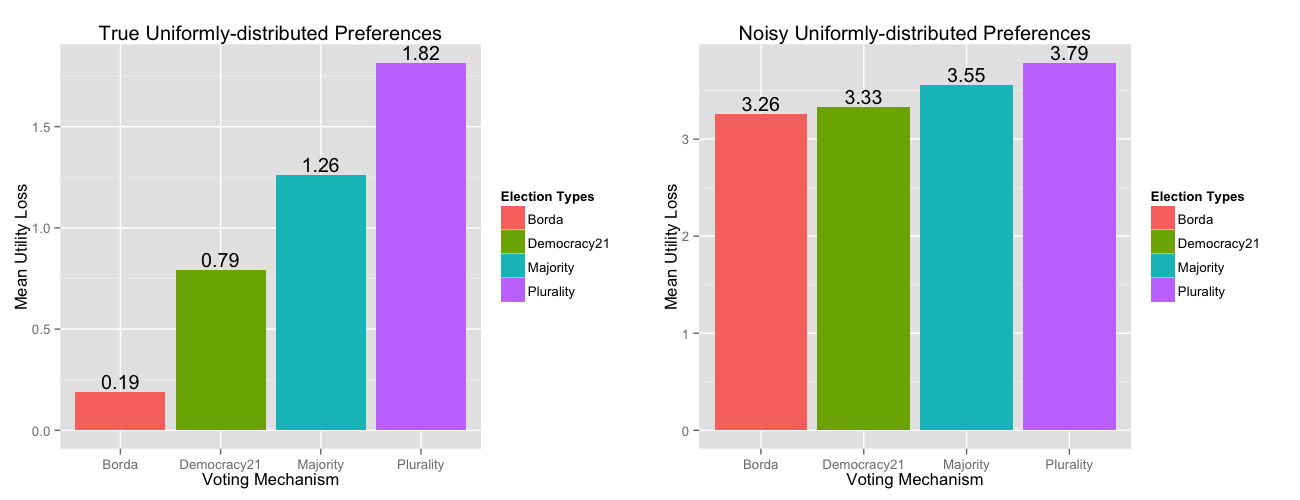
\includegraphics[scale=0.38]{uniform.png}
\caption{Bar graph of average utility losses for each election under normally distributed preferences and truthful reporting.}
\end{figure}

\begin{figure}[H]\center
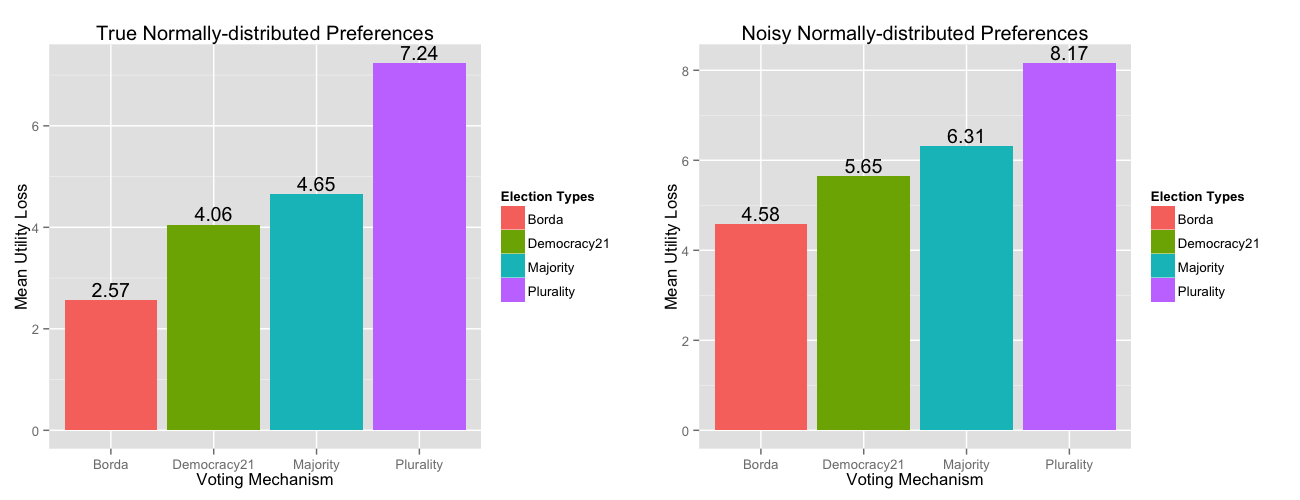
\includegraphics[scale=0.38]{normal.png}
\caption{Bar graph of average utility losses for each election under normally distributed preferences and truthful reporting.}
\end{figure}

\subsection{Tight Elections}

\begin{figure}[H]\center
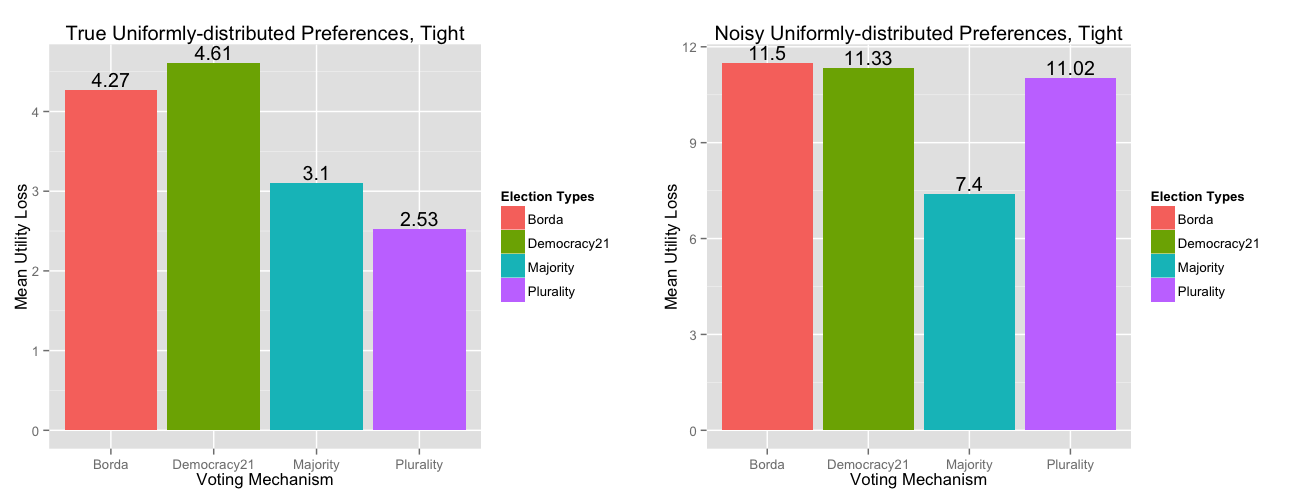
\includegraphics[scale=0.38]{uniform_tight.png}
\caption{Bar graph of average utility losses for each election under normally distributed preferences and truthful reporting.}
\end{figure}

\begin{figure}[H]\center
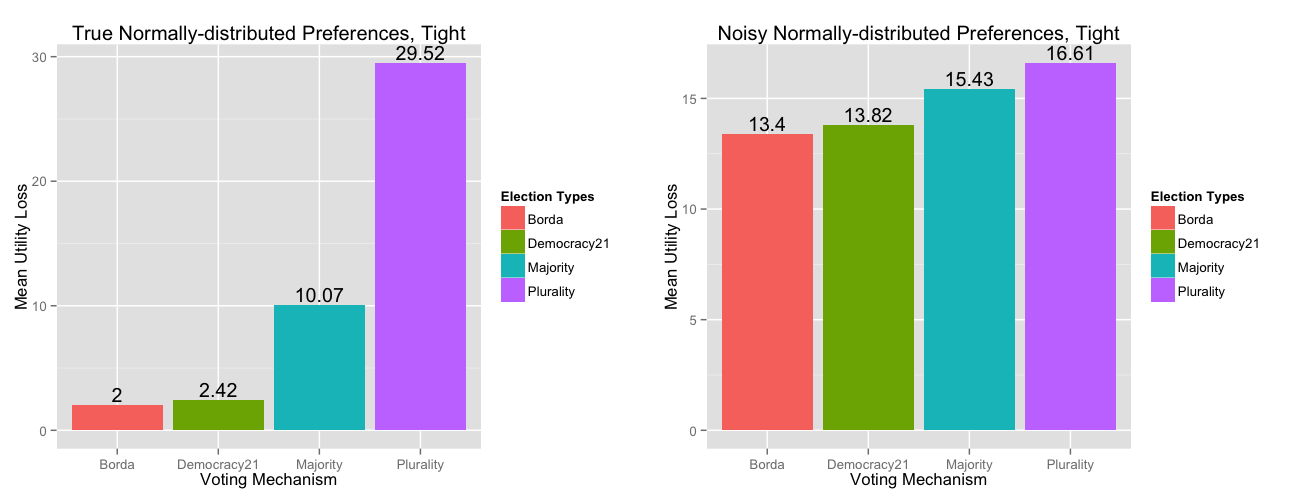
\includegraphics[scale=0.38]{normal_tight.png}
\caption{Bar graph of average utility losses for each election under normally distributed preferences and truthful reporting.}
\end{figure}


\section{Final Remarks}



\end{document}




